% Faculty-format thesis candidate (WP7-F3).
% Clean A4 layout: no official faculty template was available in the repository.
% Scientific claim boundaries remain those of docs/thesis/FINAL_CLAIM_MATRIX.md.
\documentclass[11pt,a4paper]{report}
\usepackage[margin=25mm]{geometry}
\usepackage{booktabs}
\usepackage{longtable}
\usepackage{graphicx}
\usepackage{hyperref}
\usepackage{amsmath}
\usepackage{setspace}
\usepackage{array}
\usepackage{xcolor}
\graphicspath{{../../results/figures/}{../../results/final/stage_d/figures/}}
\hypersetup{colorlinks=true,linkcolor=black,citecolor=black,urlcolor=blue}
\begin{document}

% ---------------------------------------------------------------------------
% Title page
% ---------------------------------------------------------------------------
\begin{titlepage}
\centering
{\large Technische Universit\"at Bergakademie Freiberg}\\[0.4em]
{\large Faculty of Mechanical, Process and Energy Engineering}\\[0.3em]
{\large Institute of Mechanics and Fluid Dynamics}\\[0.2em]
{\large Chair of Applied Mechanics -- Solid Mechanics}\\[2.2em]

{\LARGE\bfseries Application of Built-in Adaptive Remeshing and Mesh
Refinement Features in Abaqus to Fracture Simulations Using Phase-field
User Elements\par}
\vspace{1.2em}
{\large Master Thesis}\\[0.4em]
{\large Master of Science}\\[0.3em]
{\large Course of study: Master Computational Materials Science}\\[2.0em]

\begin{tabular}{@{}ll@{}}
\textbf{Author} & Pruthviraja Reddy Vandavagali \\
\textbf{Matriculation number} & 68865 \\
\end{tabular}\\[1.6em]

\begin{tabular}{@{}p{0.42\textwidth}p{0.48\textwidth}@{}}
\textbf{1st Examiner (Supervisor)} &
Prof.\ Dipl.-Ing.\ Bj\"orn Kiefer, Ph.D. \\[0.6em]
\textbf{2nd Examiner (Reviewer)} &
Dr.-Ing.\ Stephan Roth \\
\end{tabular}\\[2.0em]

\begin{tabular}{@{}ll@{}}
\textbf{Date of issue} & 13 July 2026 \\
\textbf{Submission deadline} & 12 January 2027 \\
\end{tabular}\\[2.2em]

{\small Running title: Adaptive Remeshing, MISESERI Refinement, and State
Transfer for Phase-Field Fracture in Abaqus}\\[0.8em]
{\small Faculty-format candidate generated from the frozen scientific
closeout (WP7-F3). Submission date is taken from the assignment sheet only
after final human/administrative clearance.}
\end{titlepage}

\pagenumbering{roman}
\tableofcontents
\clearpage
\listoffigures
\clearpage
\listoftables
\clearpage

% ---------------------------------------------------------------------------
% Abstract
% ---------------------------------------------------------------------------
\chapter*{Abstract}
\addcontentsline{toc}{chapter}{Abstract}
Phase-field fracture models implemented as Abaqus user elements (UEL/UMAT)
enable regularized crack evolution, but production use on non-uniform meshes
raises three coupled questions: whether a published staggered baseline can be
reproduced with defensible reaction-force evidence; whether offline
MISESERI-driven pre-refinement can recover peak and pre-peak response at lower
cost than a uniform production mesh; and whether nonmatching state transfer
supports a controlled pre-peak checkpoint without overstating restart or
parallel claims.

This thesis documents a staged Abaqus workflow built around the Molnar and
Gravouil staggered single-notch benchmark~\cite{molnar2017}, phase-field
implementation context from related UEL literature~\cite{msekh2015,diddige2025},
and MISESERI pre-refinement practice motivated by Pandey and
Kumar~\cite{pandey2025}. Uniform mesh roles were fixed after supervisor
decisions that accept H2-PUB for fine RF--U validation, H1 for production
comparisons, and H0 for development. Offline refinement then produced a
corrected locally refined mesh with 14.7\% fewer physical elements than H1,
close peak/pre-peak RF--U agreement, and measured wall-time and memory savings
under a fair four-thread comparison. Controlled analytical transfer, Abaqus
ingestion, serial continuation, and a bounded pre-peak nonmatching release hold
were demonstrated; an offline active-set correction at a later checkpoint was
shown to be KKT-admissible under frozen history.

The same evidence sets hard limits. Unrestricted post-peak RF--U convergence
and crack-path mesh independence are not supported. Fixed active-set
continuation under further loading is disproven in the tested segment. The
D3D-A1 corrected package is not an accepted mechanically equilibrated restart.
Threaded shared-state characterization (P3-T4) produced no threaded evidence;
MPI and hybrid safety remain unqualified. ABAQUSER equivalence remains
externally blocked. Validated online adaptive remeshing is not claimed.

Practically, the work identifies where pre-refinement and pre-peak state
transfer are usable, quantifies accuracy/cost benefits within those scopes, and
provides a decision tree that blocks unsupported post-peak, restart, and
parallel generalizations.

\clearpage
\pagenumbering{arabic}

% ---------------------------------------------------------------------------
% Body (frozen scientific chapters)
% ---------------------------------------------------------------------------
\chapter{Stage A Molnar Single-Notch Benchmark}

\section{Objective and Decision Boundary}

Stage A establishes whether the Molnar and Gravouil single-notch phase-field
benchmark is a defensible baseline for later Abaqus adaptive-remeshing work.
The aim is deliberately narrower than the full thesis workflow: reproduce an
established staggered phase-field implementation, quantify the reconstructed
single-notch response, and decide whether the evidence is strong enough to
authorize Stage B uniform-reference studies.

The current Stage A status is:

\begin{quote}
\texttt{candidate v2: technically passed}\\
\texttt{scientific review: incomplete}\\
\texttt{SDV15: completed-increment irreversibility violation}\\
\texttt{Gate A3: reference\_data\_insufficient}\\
\texttt{new solution run: not authorized}
\end{quote}

This chapter therefore treats candidate v2 as a technically reproducible and
useful reproduction baseline, but not as a Gate A3 pass. Supervisor approval is
required before any Stage B, uniform-reference, MISESERI, remeshing, or state
transfer work begins.

\section{Benchmark Choice}

The Molnar single-notch benchmark was selected because it connects directly to
the thesis requirement for an Abaqus UEL/UMAT phase-field workflow. The source
package contains a staggered displacement/phase implementation, a visualization
layer through state variables, and single-notch examples suitable for checking
reaction force, crack-path geometry, and phase-field/history behavior before
introducing adaptive remeshing.

The benchmark is also a useful stress test for thesis discipline. It separates
technical execution from scientific validation: a model can compile, solve, and
produce a plausible crack while still failing a strict scientific gate because
the RF--U reference, tolerances, or irreversibility interpretation remain
unresolved.

\section{Formulation Convention}

The phase-field convention used throughout Stage A is:

\begin{itemize}
\item \(d=0\): intact material.
\item \(d=1\): fully broken material.
\end{itemize}

Candidate v2 preserves the published Molnar source formulation. The generated
source copy \path{models/generated/molnar_gravouil_2017/paper_matched_single_notch_v2/SingleNotch_v2.for}
is copied from the preserved source with only the physical-element count
\texttt{N\_ELEM=33852} updated for the reconstructed mesh. The original source
is preserved at
\path{models/baseline_original/molnar_gravouil_2017/02_Single_Notch_Tension/SingleNotch.for}.

\section{Staggered Phase/Displacement Method}

The implementation follows a staggered solution structure with displacement
and phase-field layers. The displacement field is solved in the mechanical
layer, and the phase-field layer updates the scalar damage variable using the
stored history information. Visualization variables are copied into a companion
UMAT/CPS4 layer; those visualization fields are evidence outputs, not separate
governing fields.

For thesis use, three distinctions must remain visible:

\begin{itemize}
\item The published formulation is the Molnar and Gravouil staggered
phase-field UEL/UMAT implementation.
\item The reconstructed implementation is the project candidate-v2
paper-matched deck generated from documented geometry, loading, material, and
mesh assumptions.
\item The approximate Fig.~7 reference is a local digitization of the published
curve, not exact author data and not a supervisor-approved final tolerance
basis.
\end{itemize}

\section{Geometry, Material, and Loading}

Candidate v2 reconstructs a \(1.0~\mathrm{mm}\times1.0~\mathrm{mm}\)
single-edge-notched plate with a left-edge split-node notch of length
\(0.5~\mathrm{mm}\) at \(y=0\). The model uses plane strain and unit
thickness. Material parameters are \(E=210~\mathrm{kN/mm^2}\), \(\nu=0.3\),
\(G_c=0.0027~\mathrm{kN/mm}\), and \(l_c=0.0075~\mathrm{mm}\).

The load angle is \(90^\circ\). The loading is applied in two direct-increment
steps:

\begin{center}
\begin{tabular}{lrrr}
\toprule
Step & Start \(U_2\) (mm) & End \(U_2\) (mm) & Increment (mm) \\
\midrule
Step 1 & 0.0000 & 0.0050 & \(1.0\times10^{-5}\) \\
Step 2 & 0.0050 & 0.0067 & \(1.0\times10^{-5}\) \\
\bottomrule
\end{tabular}
\end{center}

\section{Paper-Matched Reconstruction}

The reconstruction is documented in the project configuration and derived
reference records. Candidate v2 restores the intended loading arithmetic,
implements a split-node notch, preserves the layered UEL/UMAT architecture,
and uses the source property layout from the preserved Molnar files. Static
validation passed, and the mesh-quality preflight classified the model as
\texttt{mesh\_quality\_preflight\_pass}.

The mesh has \(33852\) physical elements and \(101556\) layered elements. The
local mesh size is \(h=0.001~\mathrm{mm}\), giving \(h/l=0.1333333333\). The
maximum element size is \(0.025~\mathrm{mm}\), the maximum neighboring-size
ratio is \(1.5\), and the maximum aspect ratio is \(25.000000000001368\). The
high-aspect-ratio elements are documented as reconstruction limitations outside
the fracture-process corridor.

\section{Technical Validation}

The single authorized serial HPC baseline job was
\texttt{1374864.mmaster02}, submitted from revision
\texttt{711dd495bdcb830d695f9d7e56283316c9d417d5}. It completed with PBS
\texttt{Exit\_status=0}; Abaqus returned code zero; the \texttt{.sta},
\texttt{.msg}, \texttt{.dat}, and scratch \texttt{.odb} outputs existed; and
the \texttt{.sta} reported successful analysis completion. The technical
classification is \texttt{paper\_matched\_v2\_technical\_pass}.

The run used one CPU, \(32~\mathrm{GB}\) requested memory, and a 24-hour
walltime request. Recorded resource use was walltime \(00{:}38{:}38\), CPU
time \(00{:}35{:}52\), CPU percent \(95\), memory \(2970760~\mathrm{kb}\),
virtual memory \(3565868~\mathrm{kb}\), and an Abaqus-reported peak memory of
about \(2~\mathrm{GB}\).

\section{Numerical Results}

\begin{longtable}{p{0.40\linewidth}p{0.25\linewidth}p{0.27\linewidth}}
\caption{Stage A candidate-v2 numerical evidence. Values are drawn from
committed extraction, scientific-review, and targeted-diagnostic evidence.}\\
\toprule
Metric & Value & Evidence \\
\midrule
\endfirsthead
\toprule
Metric & Value & Evidence \\
\midrule
\endhead
Peak RF2 & \(0.761702~\mathrm{kN}\) & \path{runs/hpc/paper_matched_single_notch_v2/scientific_review/fig7_comparison_metrics.json} \\
Peak displacement & \(U_2=0.006110~\mathrm{mm}\) & \path{runs/hpc/paper_matched_single_notch_v2/scientific_review/fig7_comparison_metrics.json} \\
Peak-force error & \(0.064519\) relative & \path{runs/hpc/paper_matched_single_notch_v2/scientific_review/FIG7_COMPARISON_AUDIT.md} \\
Peak-displacement error & \(0.041257\) relative & \path{runs/hpc/paper_matched_single_notch_v2/scientific_review/FIG7_COMPARISON_AUDIT.md} \\
Pre-peak RMSE & \(0.044136~\mathrm{kN}\) & \path{runs/hpc/paper_matched_single_notch_v2/scientific_review/FIG7_COMPARISON_AUDIT.md} \\
Post-peak RMSE & \(0.348093~\mathrm{kN}\) & \path{runs/hpc/paper_matched_single_notch_v2/scientific_review/FIG7_COMPARISON_AUDIT.md} \\
Full-overlap NRMSE & \(0.245705\) & \path{runs/hpc/paper_matched_single_notch_v2/scientific_review/fig7_comparison_metrics.json} \\
Tangent-stiffness error & about \(+51.4\%\) & \path{runs/hpc/paper_matched_single_notch_v2/scientific_review/SCIENTIFIC_DECISION.md} \\
Common-domain area error & \(+0.193324\) relative & \path{runs/hpc/paper_matched_single_notch_v2/scientific_review/fig7_comparison_metrics.json} \\
Crack extension, SDV15 \(\ge0.80\) & \(0.0555~\mathrm{mm}\) beyond notch tip; \(0.0570~\mathrm{mm}\) total connected path & \path{runs/hpc/paper_matched_single_notch_v2/scientific_review/SCIENTIFIC_DECISION.md} \\
Crack extension, SDV15 \(\ge0.90\) & \(0.0525~\mathrm{mm}\) beyond notch tip; \(0.0530~\mathrm{mm}\) total connected path & \path{runs/hpc/paper_matched_single_notch_v2/scientific_review/SCIENTIFIC_DECISION.md} \\
Crack extension, SDV15 \(\ge0.95\) & \(0.0505~\mathrm{mm}\) beyond notch tip; \(0.0510~\mathrm{mm}\) total connected path & \path{runs/hpc/paper_matched_single_notch_v2/scientific_review/SCIENTIFIC_DECISION.md} \\
Crack extension, SDV15 \(\ge0.99\) & \(0.0465~\mathrm{mm}\) beyond notch tip; \(0.0460~\mathrm{mm}\) total connected path & \path{runs/hpc/paper_matched_single_notch_v2/scientific_review/SCIENTIFIC_DECISION.md} \\
SDV15 maximum overshoot & \(1.005600\) & \path{runs/hpc/paper_matched_single_notch_v2/scientific_review/sdv_irreversibility_metrics.json} \\
Accepted-increment decreasing transitions & \(2184\) & \path{runs/hpc/paper_matched_single_notch_v2_sdv15_diagnostic_r2/RUN_SUMMARY.md} \\
Transitions above \(10^{-6}\) & \(2131\) & \path{runs/hpc/paper_matched_single_notch_v2_sdv15_diagnostic_r2/evidence/1375028.mmaster02/postprocessing_completed_increment_replay_time_aligned/severity_audit/sdv15_completed_increment_severity_summary.json} \\
Transitions above \(10^{-5}\) & \(1362\) & \path{runs/hpc/paper_matched_single_notch_v2_sdv15_diagnostic_r2/evidence/1375028.mmaster02/postprocessing_completed_increment_replay_time_aligned/severity_audit/sdv15_completed_increment_severity_summary.json} \\
Maximum decrease & \(2.2384088238425193\times10^{-4}\) & \path{runs/hpc/paper_matched_single_notch_v2_sdv15_diagnostic_r2/RUN_SUMMARY.md} \\
Mean decrease & \(2.8434597987446906\times10^{-5}\) & \path{runs/hpc/paper_matched_single_notch_v2_sdv15_diagnostic_r2/RUN_SUMMARY.md} \\
Median decrease & \(1.3940791172561973\times10^{-5}\) & \path{runs/hpc/paper_matched_single_notch_v2_sdv15_diagnostic_r2/RUN_SUMMARY.md} \\
Unique affected element/IP locations & \(138\) & \path{runs/hpc/paper_matched_single_notch_v2_sdv15_diagnostic_r2/RUN_SUMMARY.md} \\
SDV16 decreases & \(0\) & \path{runs/hpc/paper_matched_single_notch_v2_sdv15_diagnostic_r2/RUN_SUMMARY.md} \\
Diagnostic RF--U perturbation & maximum normalized RF2 difference \(6.54442468760855\times10^{-13}\); maximum U2 difference \(4.992967844730245\times10^{-15}~\mathrm{mm}\) & \path{runs/hpc/paper_matched_single_notch_v2_sdv15_diagnostic_r2/RUN_SUMMARY.md} \\
Solver walltime and memory & baseline PBS walltime \(00{:}38{:}38\), memory \(2970760~\mathrm{kb}\), Abaqus peak memory about \(2~\mathrm{GB}\) & \path{runs/hpc/paper_matched_single_notch_v2/scientific_review/solver_resource_metrics.json} \\
\bottomrule
\end{longtable}

\section{RF--U Interpretation}

The RF--U comparison is mixed. The peak force scale is close enough to justify
continued review, but the full curve is not within a strict provisional
working gate. The pre-reference-peak RMSE is \(0.044136~\mathrm{kN}\), while
the post-reference-peak RMSE is \(0.348093~\mathrm{kN}\). This makes the
post-peak mismatch the dominant scientific limitation. The comparison uses the
approximate digitized Fig.~7 red dashed \(l_c=0.0075~\mathrm{mm}\) reference,
which has estimated digitization uncertainty of about
\(\pm0.00004~\mathrm{mm}\) and \(\pm0.015~\mathrm{kN}\).

\section{Crack-Path Interpretation}

The final high-damage band is connected and approximately horizontal at
thresholds from \(\mathrm{SDV15}\ge0.80\) through
\(\mathrm{SDV15}\ge0.99\). At the provisional
\(\mathrm{SDV15}\ge0.95\) threshold, the final matched contour contains
193 element-mean damaged elements and a connected high-damage extension of
about \(0.0505~\mathrm{mm}\) beyond the notch tip. This supports qualitative
crack-direction agreement, but it remains threshold-dependent and does not
close Gate A3 by itself.

\section{SDV15, SDV16, and Irreversibility}

In the project convention, SDV15 is the phase-field visualization variable and
SDV16 is the history-like variable used to monitor monotonic driving behavior.
The original ODB scan found SDV16 monotone and SDV15 nonmonotone in retained
visualization frames. A later targeted diagnostic r2 run was non-intrusive by
RF--U comparison and enabled a no-solution completed-increment replay of the
existing trace rows.

The completed-increment replay kept the last U1 stage-101 call for each
\((\mathrm{KSTEP}, \mathrm{KINC}, \mathrm{physical~element},
\mathrm{source-storage~IP})\). It processed 627304 trace rows, retained
209152 U1 stage-101 rows, formed 101840 final increment states over 152
element/IP sequences, and found 2184 unique completed-increment SDV15
decreasing transitions. The severity audit classifies this as
\texttt{sdv15\_completed\_increment\_irreversibility\_violation} under the
provisional \(10^{-6}\) materiality tolerance. SDV16 has zero decreases over
the same final-increment sequences.

\section{Scientific Limitations}

The current evidence supports the following restrained interpretation:

\begin{itemize}
\item Candidate v2 is technically reproducible.
\item Crack propagation direction is qualitatively correct.
\item RF--U agreement is mixed, and post-peak disagreement is substantial.
\item SDV16 remains monotone in the checked sequences.
\item SDV15 decreases between accepted increments.
\item The targeted diagnostic instrumentation is non-intrusive.
\item Strict pointwise phase-field irreversibility is not satisfied.
\item Candidate v2 remains a useful reproduction baseline for supervisor
review.
\item Supervisor approval is required before Stage B or any downstream
adaptive-remeshing work.
\end{itemize}


\section{Supplementary lc = 0.015 mm mesh h-convergence (RF--U)}
\label{sec:lc015-hconv-thesis}

For the exact author-supplied supplementary single-notch model (\(l_c=0.015\,\mathrm{mm}\)), three serial meshes were solved and postprocessed for RF--U only.
Successive peak-force changes are approximately \(4.0\%\) (H0\(\to\)H1) and \(0.47\%\) (H1\(\to\)H2-PUB); pre-peak curve NRMSE between H1 and H2-PUB is about \(0.11\%\), while post-peak residual remains larger (\(\sim 20\%\) NRMSE).
After supervisor Decisions~\textbf{1A} and \textbf{2B}, mesh roles are frozen as:
H2-PUB for fine RF--U validation only; H1 for production/thesis/report simulations and the Stage~C comparison reference; H0 for fast testing and the first MISESERI implementation trials.
Crack-path/contour mesh convergence remains deferred (Decision~\textbf{2B}) and does not block Stage~C preparation.
Evidence: \path{runs/hpc/molnar_lc015_h_convergence/comparison/H_CONVERGENCE_SCIENTIFIC_REVIEW.md};
\path{docs/decisions/MOLNAR_GATE_A3_SUPERVISOR_DECISION_1A_2B.md};
\path{docs/decisions/MESH_USE_POLICY.md}.

\section{Gate A3 Boundary}

Gate A3 is \textbf{conditionally accepted for RF--U validation use} after Decisions~\textbf{1A} and \textbf{2B}
(\texttt{gate\_a3\_conditionally\_accepted\_rf\_u}; \texttt{contour\_validation\_deferred}).
Full unconditional closure of every historical Stage~A claim is not asserted; residual items may still retain a
\texttt{reference\_data\_insufficient} narrative where appropriate.
Candidate v2 has not been reclassified as a full scientific pass by these decisions.
Stage~C MISESERI \textbf{preparation} is authorized; HPC submission, MISESERI execution, multicore qualification,
and state-transfer work remain unauthorized without explicit further approval.
Stage~C preparation plan: \path{docs/studies/STAGE_C_MISESERI_PREPARATION_PLAN.md}.

\chapter{Representative Results and Evidence Figures}
\label{chap:key-figures}

This chapter collects the five representative figures required for the
faculty-format package. Captions preserve the frozen claim boundaries: peak and
pre-peak RF--U findings are supported; unrestricted post-peak convergence,
crack-path mesh independence, accepted D3D-A1 mechanical restart, ABAQUSER
equivalence, and validated online adaptive remeshing are not claimed.

\section{Baseline reaction response}

\begin{figure}[htbp]
\centering
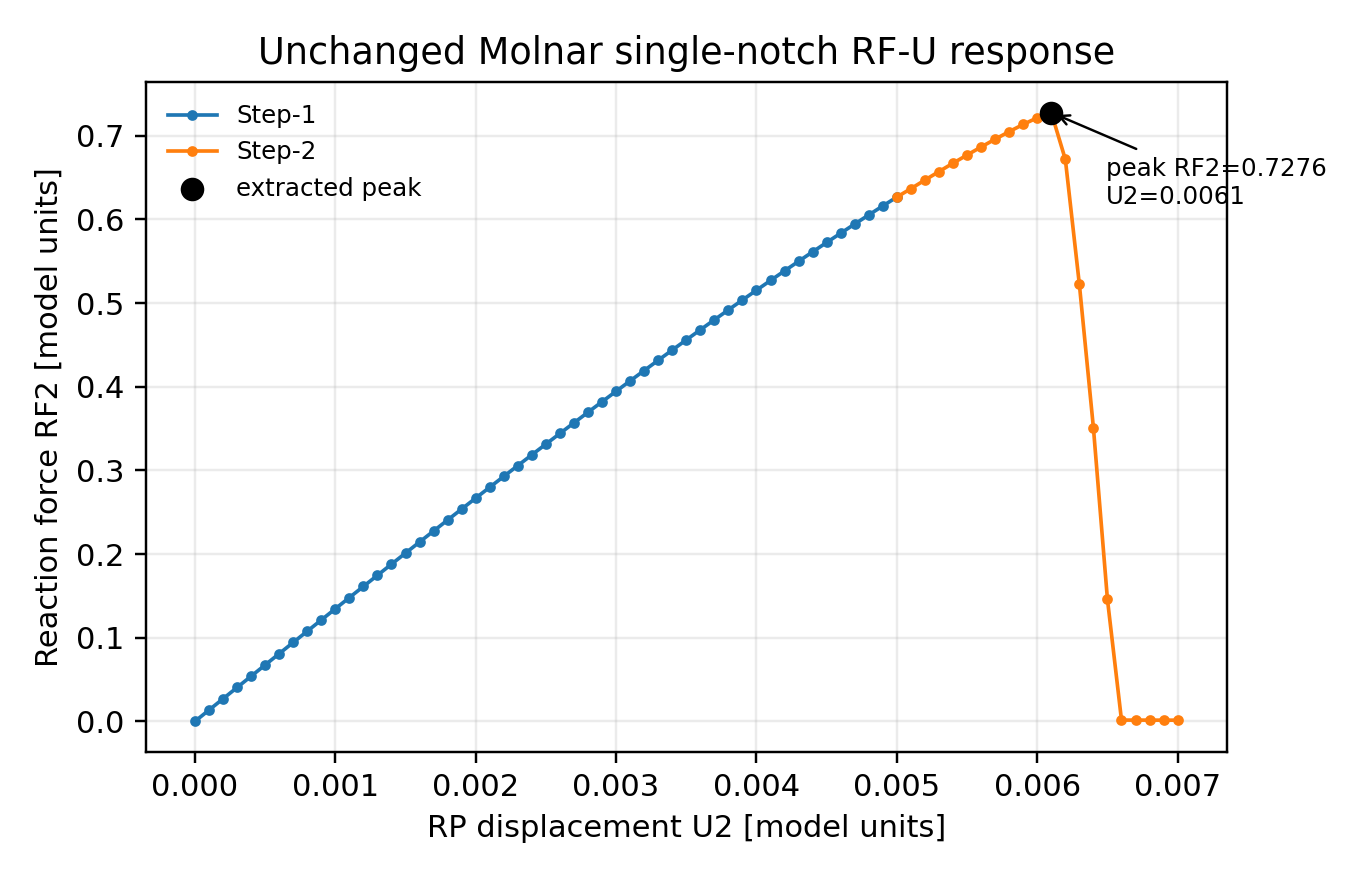
\includegraphics[width=0.92\textwidth]{stage_a_baseline/single_notch_rf_u_curve.png}
\caption{Representative single-notch RF--U curve extracted from the Stage~A
paper-matched baseline workflow. The figure supports technical reproducibility
of the Molnar-type staggered response~\cite{molnar2017}; it does not by itself
establish unrestricted Gate~A3 scientific closure or post-peak mesh
independence.}
\label{fig:baseline-rf-u}
\end{figure}

\section{Uniform-mesh RF--U comparison}

\begin{figure}[htbp]
\centering
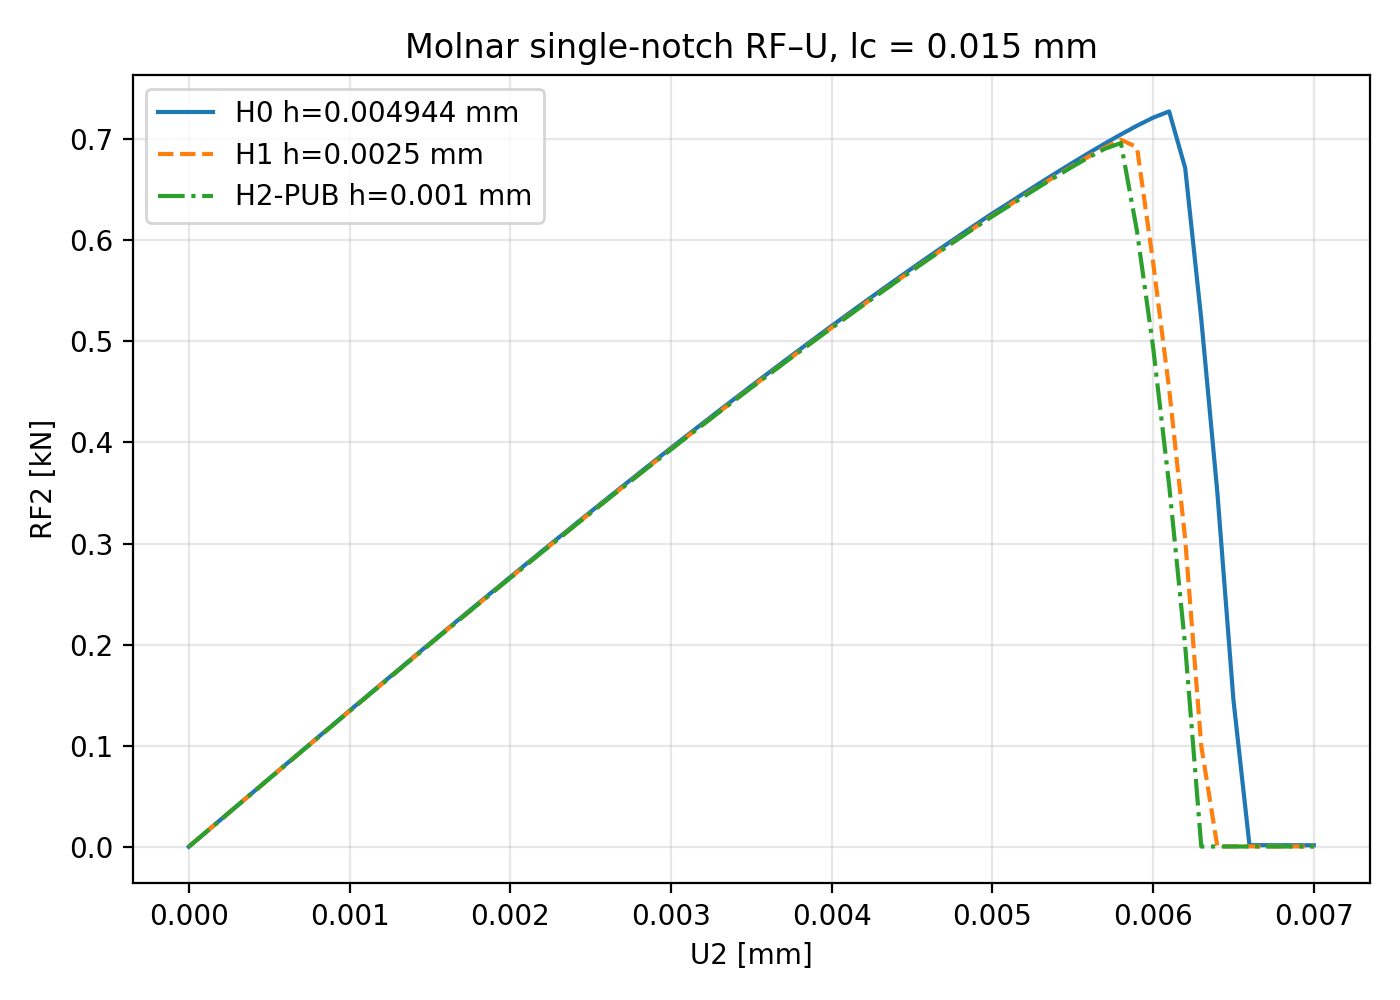
\includegraphics[width=0.92\textwidth]{molnar_lc015_h_convergence/01_rf_u_h0_h1_h2.png}
\caption{RF--U comparison for the supplementary \(l_c=0.015\,\mathrm{mm}\)
uniform meshes H0, H1, and H2-PUB. Peak and pre-peak agreement underpins the
supervisor mesh roles (H2-PUB validation, H1 production, H0 development). Larger
post-peak residual differences remain a stated limitation.}
\label{fig:rf-u-h-convergence}
\end{figure}

\section{Offline MISESERI refinement comparison}

\begin{figure}[htbp]
\centering
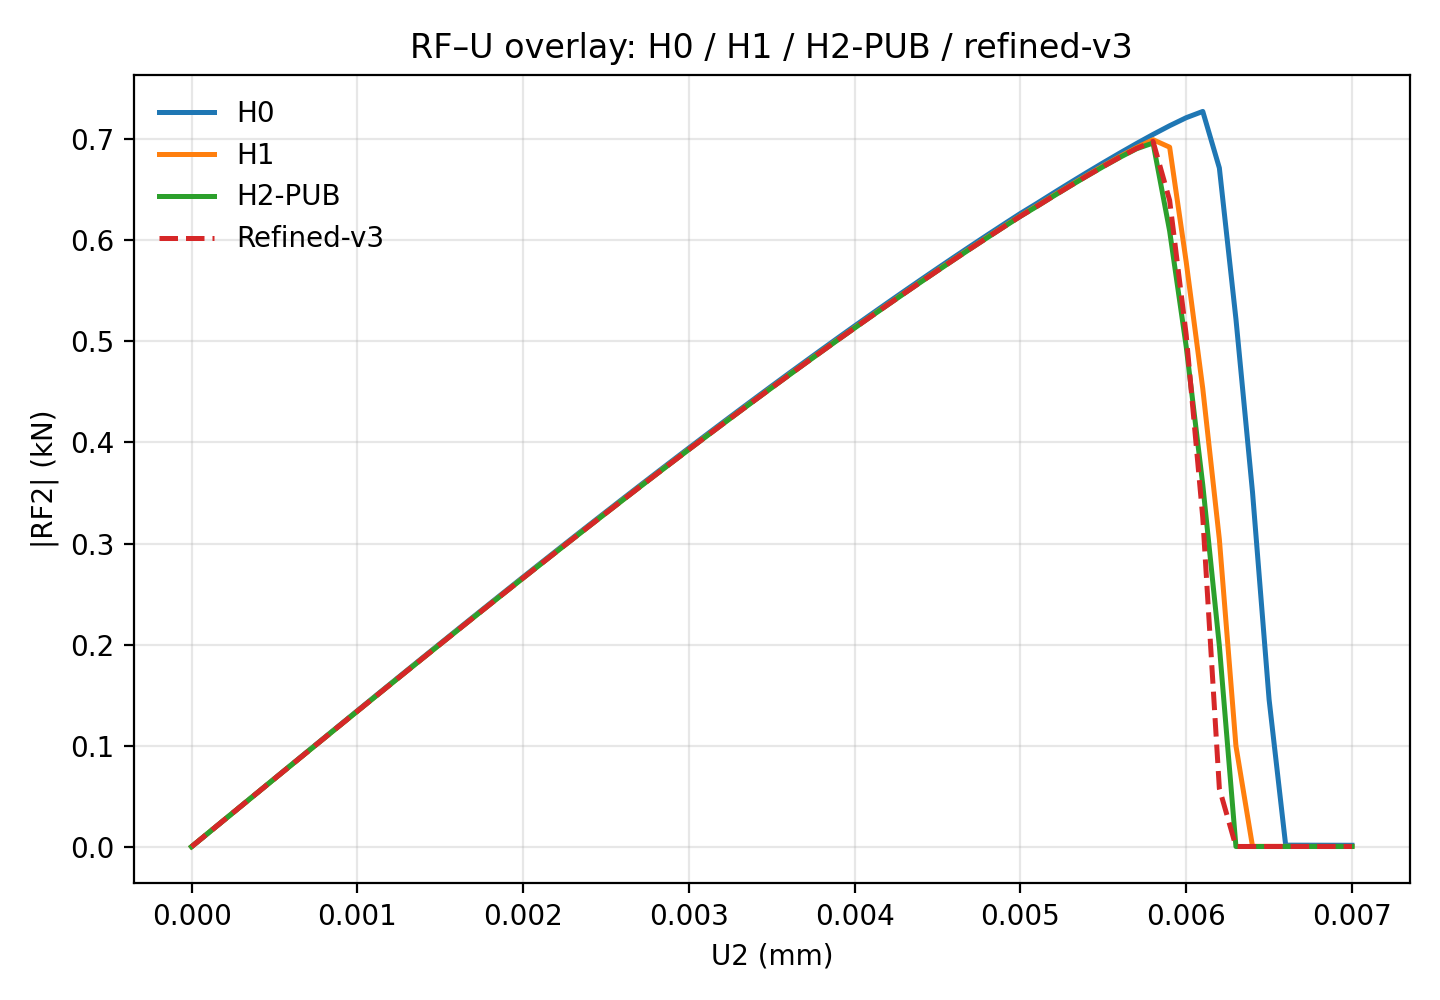
\includegraphics[width=0.92\textwidth]{stage_c_final/01_rf_u_h0_h1_h2_refined_v3.png}
\caption{RF--U comparison of the Stage~C corrected offline refined mesh against
the uniform references. The refined model is supported for elastic, pre-peak,
and peak RF--U response within the tested parameter set~\cite{pandey2025}, not
as a post-peak crack-path-equivalent replacement for H1.}
\label{fig:miseseri-refined-rf-u}
\end{figure}

\section{Stage~D transfer workflow evidence}

\begin{figure}[htbp]
\centering
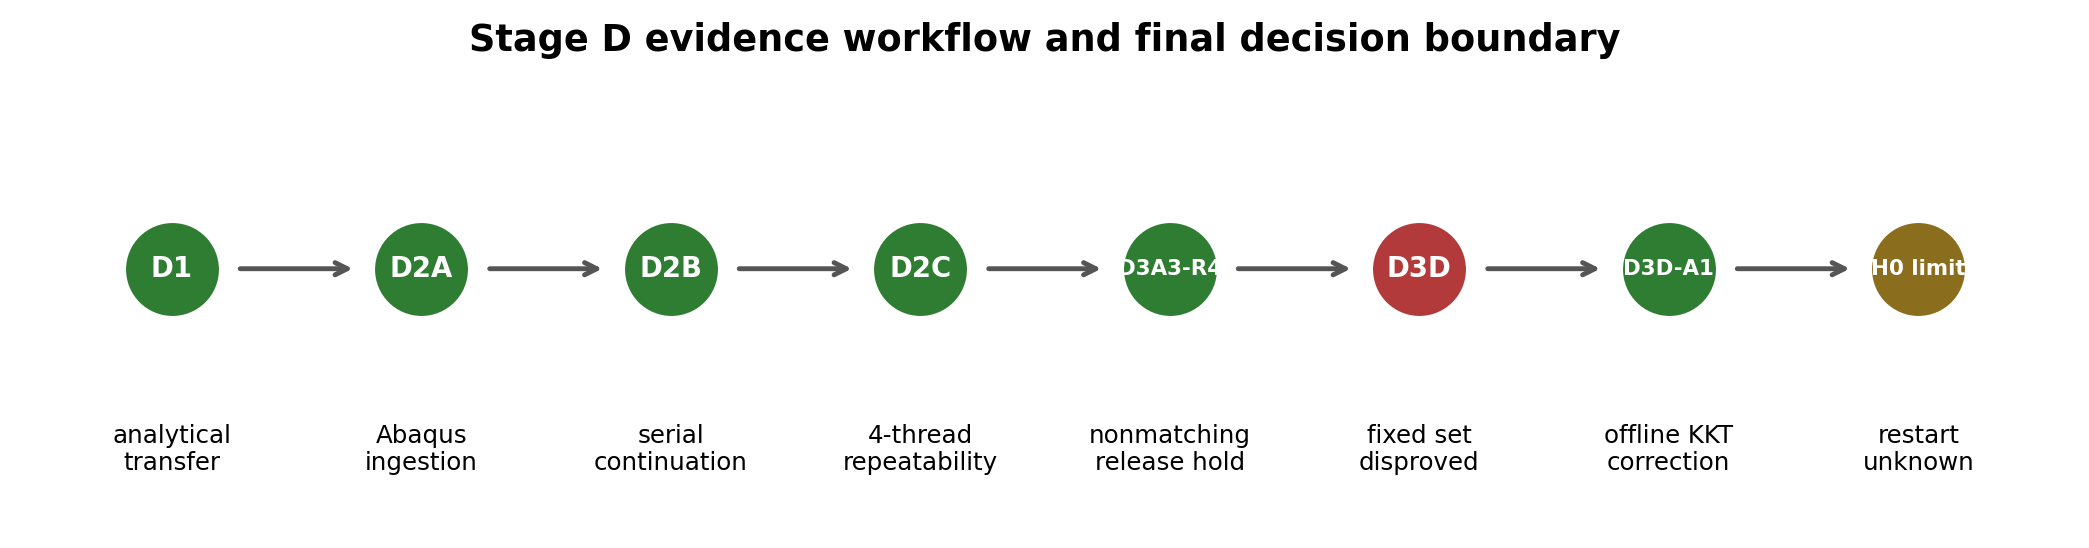
\includegraphics[width=0.88\textwidth]{stage_d_workflow.png}
\caption{Stage~D transfer workflow summary from the final synthesis package.
Controlled field transfer, Abaqus ingestion, serial continuation, and the
bounded pre-peak release hold are within scope; online remeshing continuation
is not claimed.}
\label{fig:stage-d-workflow}
\end{figure}

\section{Active-set limitation evidence}

\begin{figure}[htbp]
\centering
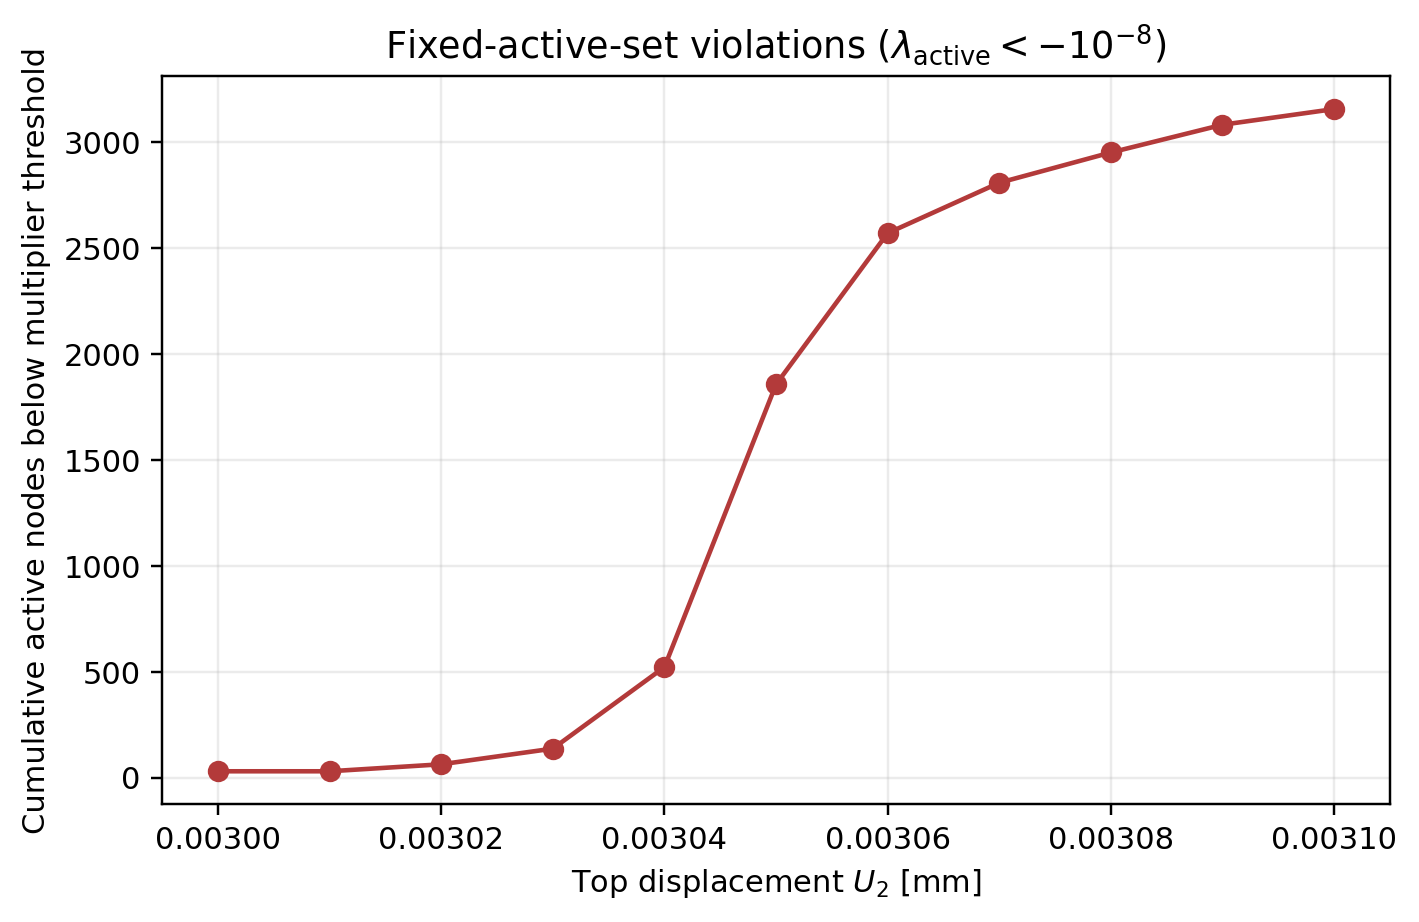
\includegraphics[width=0.92\textwidth]{violating_active_nodes_vs_displacement.png}
\caption{Count of active-set multiplier violations versus displacement in the
D3D continuation segment. The trend disproves a fixed active set under further
loading in the tested range and motivates offline correction without elevating
the D3D-A1 candidate to an accepted mechanical restart.}
\label{fig:active-set-limitation}
\end{figure}

% Thesis chapter draft: Stage C offline refinement demonstration.
\chapter{Offline MISESERI Pre-Refinement for Layered Phase-Field UEL Models}
\label{ch:stage-c-offline-refinement}

\section{Objective}
Demonstrate a custom, auxiliary-continuum, MISESERI-driven offline pre-refinement
workflow for the Molnar layered phase-field UEL model, targeting the elastic,
pre-peak and peak RF--U response of uniform H1 with fewer physical elements.

\section{Method summary}
\begin{enumerate}
  \item Solve an auxiliary continuum pre-analysis with active MISESERI output.
  \item Mark elements with
  \[
    \frac{\mathrm{MISESERI}}{\max(\mathrm{MISESERI})}
    > \texttt{relative\_MISESERI\_threshold},\qquad
    \texttt{relative\_MISESERI\_threshold}=0.05.
  \]
  \item Build a localized graded physical mesh (min size $0.0025\,\mathrm{mm}$,
  max size $0.025\,\mathrm{mm}$, one pass, no coarsening).
  \item Reconstruct U1/U2/CPS4 layers and Fortran \texttt{N\_ELEM}.
  \item Solve with four OpenMP threads and compare to uniform H1.
\end{enumerate}

\section{Verification narrative}
A failed iteration (C2F-v2) omitted the exact $y=0$ mesh line, so notch free faces
were not reconstructed. The resulting continuous plate elevated initial stiffness
by about $72\%$ and suppressed softening. Geometry audit, restoration of $y=0$,
elastic probe ($0.083\%$ stiffness error), phase-field spatial check, and C2F-v3
restored peak/pre-peak agreement with H1.

\section{Results (C2F-v3)}
Peak force difference $0.24\%$; initial stiffness difference $0.061\%$;
pre-peak NRMSE $0.089\%$; peak displacement identical at $0.0058\,\mathrm{mm}$;
$10290$ physical elements ($14.7\%$ fewer than H1). Post-peak NRMSE remains about
$24\%$ and is reported as limited equivalence only.

\section{Production policy}
Uniform H1 remains the production and report reference. The refined mesh is a
demonstration of offline pre-refinement efficiency, not a replacement of H1.
Fair walltime comparisons require a four-thread H1 baseline.

% Thesis chapter draft: Stage D controlled state transfer.
\chapter{Controlled State Transfer for Phase-Field UEL Workflows}
\label{ch:stage-d-state-transfer}

\section{Objective}
Stage D tests whether phase-field and history values transferred between meshes
are actually ingested by Abaqus and routed through the UEL/UMAT state arrays.
The test is intentionally separated from fracture evolution. No interrupted
Molnar fracture simulation is allowed until the D2 ingestion, continuation,
thread-repeatability, and output-routing gates pass.

\section{D1 analytical baseline}
The D1 harness established deterministic and physically guarded transfer
mechanics, but it did not prove negligible transfer error. The retained D1
baselines are:

\begin{table}[h]
\centering
\begin{tabular}{@{}lr@{}}
\toprule
Quantity & Value \\
\midrule
Nodal $d$ L2 error & $0.0270$ \\
Nodal $d$ maximum error & $0.0850$ \\
Integration-point $H$ L2 error & $0.0108$ \\
Integration-point $H$ maximum error & $0.0234$ \\
Energy difference & $-0.00769$ \\
\bottomrule
\end{tabular}
\end{table}

\section{D2A ingestion design}
D2A uses the prepared tiny nonmatching transfer package under
\texttt{models/state\_transfer/d2\_tiny\_transfer/}. A separate D2-only
UEL/UMAT source variant is generated under
\texttt{src/state\_transfer/d2\_tiny\_transfer\_uel.for}; the frozen Molnar
source and accepted C2C-v3 mesh are not modified.

The preserved Molnar U1 user-element card declares phase on Abaqus DOF~3. D2A
therefore prescribes every transferred nodal phase value on DOF~3 and extracts
the phase-layer nodal solution directly from the ODB. History values are loaded
from a generated read-only table keyed by physical element label and integration
point number, initialized once, and mirrored to visualization \texttt{SDV16}.
The interpolated phase value is mirrored to \texttt{SDV15}.

\section{Current status}
The executable D2A package is statically validated and ready for the first
serial ingestion job. No \texttt{D2A.ok} may be created until the Abaqus solve
exits with code zero, the ODB is readable, target-node and target element/IP
coverage are complete, and \texttt{SDV15}/\texttt{SDV16} match the independent
transfer comparison within $10^{-8}$.

\chapter{State Transfer and Active-Set Evolution}
\label{chap:stage-d-synthesis}

\section{Controlled Transfer and Abaqus Ingestion}

Stage D began with a controlled analytical transfer between nonmatching meshes.
All target nodes and integration points were mapped deterministically and the
transferred fields remained finite and bounded.  The measured nodal phase
\(L_2\) and maximum errors were \(2.7037\times10^{-2}\) and
\(8.4997\times10^{-2}\); the corresponding history errors were
\(1.0797\times10^{-2}\) and \(2.3398\times10^{-2}\).  These values are retained
as an error baseline rather than described as negligible.

The D2A Abaqus test then proved ingestion of transferred phase and history
through the visualization-layer state variables.  D2B proved a bounded serial
continuation after one documented increment-limit correction.  D2C repeated
the accepted continuation with one MPI rank and four threads.  State fields,
reaction history, energy, and increment sequence were identical to the serial
reference within the recorded comparison precision.

\section{Nonmatching Fracture Checkpoint}

The D3 route transferred a pre-peak checkpoint at
\(U_2=0.003000000026077032\,\mathrm{mm}\) to a nonmatching split-notch mesh
with 6,601 nodes, 6,400 physical elements, and 25,600 integration points.
Package validation established complete coverage, zero unmapped state records,
and no non-positive Jacobians.  The R4 compatible release-hold job
\texttt{1377471.mmaster02} then proved nonmatching state ingestion,
checkpoint equilibration, actual-history KKT consistency, irreversible
active-set release, and state retention through the bounded hold.  Maximum
SDV15 and SDV16 transfer errors were \(1.3878\times10^{-17}\) and zero;
relative RF and energy release jumps were \(2.2926\times10^{-4}\) and
\(1.2746\times10^{-5}\).

\section{Active-Set Evolution}

The fixed R4 active set was tested under a short continuation segment in D3D.
The first invalid state was already the segment initial frame: 30 active
multipliers were below the fixed threshold \(-10^{-8}\).  The count increased
to 3,157 nodes by the endpoint.  Thus, a fixed active set through further
loading was disproven within the tested segment even though free residual,
irreversibility, lower-bound, and Jacobian checks remained valid.

An offline primal--dual correction at the unchanged checkpoint used the
recovered F3 phase as lower bound and actual F3 history without modification.
It converged in seven iterations to 6,374 active and 227 free nodes.  All 30
initial seeds and 42 additional nodes were released, with no reactivation.
The free residual was \(2.1176\times10^{-21}\), the minimum active multiplier
was \(-9.99696\times10^{-9}\), active-bound error was zero, and the phase
functional decreased.  This proves mathematical admissibility under frozen F3
history.

\section{Mechanical-Restart Limitation}

The corrected candidate is not an accepted mechanical restart.  Three bounded
qualification jobs stopped before Abaqus because of execution-wrapper
environment failures: a platform-dependent checksum, Python syntax unsupported
by the default compute-node interpreter, and unavailable \texttt{git} after
module loading.  Mechanical re-equilibration and actual-history KKT
reassessment were therefore not performed.  The mechanical checkpoint
response remains unknown, and no phase release, D3E, peak/post-peak, crack-path,
or online-remeshing conclusion is drawn.

\section{Claim Summary}

\begin{table}[htbp]
\centering
\caption{Stage D evidence and claim boundary.}
\label{tab:stage-d-claims}
\begin{tabular}{p{0.52\linewidth}p{0.38\linewidth}}
\hline
Result & Status \\
\hline
Controlled field transfer & proven \\
Abaqus state ingestion & proven \\
Serial continuation after transfer & proven \\
Four-thread repeatability & proven within tested scope \\
Nonmatching checkpoint transfer & proven within bounded pre-peak scope \\
R4 release hold & proven \\
Fixed active set through further loading & disproven \\
Offline active-set correction & proven under frozen F3 history \\
Corrected mechanical restart & unproven \\
Online remeshing continuation & not claimed \\
D3E/post-peak continuation & not performed \\
\hline
\end{tabular}
\end{table}

\chapter{Interrupted-Transfer Checkpoint Correction}
\label{chap:d3d-a1-checkpoint}

\section{Methodology}

The transferred checkpoint was assessed at
\(U_2=0.003000000026077032\,\mathrm{mm}\).  The recovered F3 phase field at
6,601 nodes was retained as the irreversibility lower bound, while the 25,600
actual F3 integration-point history values were held fixed.  No mesh,
material, phase-field formulation, Fortran implementation, solver tolerance,
or loading parameter was changed.

The corrected phase field was obtained offline with a deterministic
primal--dual active-set iteration.  At each iteration, active nodes were fixed
at the recovered F3 lower bound and the reduced phase system was solved for the
free nodes.  Nodes violating the lower bound were reactivated, while active
nodes with a multiplier below \(-10^{-8}\) were released.  Acceptance required
a free residual infinity norm no greater than \(10^{-8}\), a minimum active
multiplier no smaller than \(-10^{-8}\), an active-bound error no greater than
\(10^{-10}\), complete phase/history coverage, no non-positive Jacobian
determinants, and no increase of the phase functional.

\section{Offline Correction Result}

The offline correction converged deterministically in seven iterations to
6,374 active and 227 free nodes.  The final free residual infinity norm was
\(2.1176\times10^{-21}\), the minimum active multiplier was
\(-9.99696\times10^{-9}\), and the active-bound error was zero.  The phase
functional changed by \(-1.6759\times10^{-10}\).  No phase-decrease,
history-change, lower-bound, state-reset, or non-positive-Jacobian violation
was detected.

These results establish that the corrected phase field is mathematically
admissible for the frozen F3 history under the prescribed KKT gates.  The
result classification is
\texttt{stage\_d3d\_a1\_checkpoint\_obstacle\_update\_pass}.  The associated
package contains the corrected phase, unchanged actual F3 history, original F3
lower bound, and converged 6,374/227 membership.

\section{Mechanical-Checkpoint Qualification}

The candidate package is not an accepted Abaqus restart state.  Mechanical
re-equilibration was intentionally placed behind a fixed-phase datacheck and
checkpoint-hold gate.  Three bounded datacheck attempts terminated before
Abaqus execution:

\begin{enumerate}
  \item job \texttt{1378003.mmaster02} compared a Windows-derived Fortran
        checksum with the LF-normalized Linux checkout;
  \item job \texttt{1378004.mmaster02} used Python assignment-expression
        syntax unsupported by the compute-node default Python~3.6; and
  \item job \texttt{1378005.mmaster02} reached a common preflight in which
        \texttt{git} was unavailable after the module purge/load sequence.
\end{enumerate}

None of these jobs compiled the user subroutine, processed the Abaqus input, or
completed a datacheck.  They are execution-wrapper failures and do not
contradict the offline obstacle result.  The final bounded stopping rule was
therefore applied and no further retry was authorized.

\section{Limitations}

The mechanical response of the corrected checkpoint under re-equilibrated
actual history remains unknown.  Consequently, the present evidence does not
establish mechanical continuity after correction, actual-history KKT validity
after equilibration, or an accepted continuation state.  It also provides no
basis for conclusions concerning phase release, D3E, peak load, post-peak
response, or crack-path evolution.

The unresolved checkpoint response is an execution-validation limitation, not
evidence that the offline active-set correction failed.  The corrected package
is retained as a mathematically admissible candidate state, but not as a
validated mechanical restart state.

\section{Future Work}

Any future continuation of this route requires a new execution decision rather
than a scientific-parameter correction.  A replacement workflow should
separate login-side repository checks from compute-node validation, bind every
required executable explicitly after module loading, and qualify the
environment independently before another Abaqus submission.  Until such a
decision is made, full checkpoint hold, phase release, continuation, D3E, and
tolerance changes remain prohibited.

\section{Parallel execution and shared user-subroutine state}
\label{sec:externaldb-parallelization}

The use of \texttt{UEXTERNALDB} is not, by itself, incompatible with parallel
Abaqus/Standard execution.  The callback provides analysis- and
increment-boundary points at which external data can be initialized or
exchanged.  The relevant correctness question is instead how that information
is stored and subsequently accessed by element and material subroutines.

The present implementation transfers phase and history information through
mutable Fortran \texttt{COMMON} blocks and also contains \texttt{SAVE} and
\texttt{DATA} storage.  Threads in one process share these objects, so
concurrent UEL and UMAT calls can create read--write or write--write races
unless ownership is guaranteed or access is synchronized.  Separate MPI
processes present a different problem: each rank has its own common-block
instance, and common storage therefore cannot provide inter-rank exchange.
Distributed support would require an explicit ownership and communication
design at defined synchronization points.

The earlier D2C comparison produced identical serial and one-rank/four-thread
phase, history, reaction-force, energy, and increment results.  This is
positive but case-specific evidence; it does not prove general thread safety.
Stage~P therefore isolates the question in an eight-physical-element model.
Bounded diagnostics record callback identity, rank and thread identifiers,
first access to each shared location, initialization, live writer conflicts,
and final call counts.  A serial diagnostic is the mandatory reference before
one four-thread characterization.  MPI, hybrid, and production claims remain
withheld.

The first instrumented serial package terminated before element execution
because \texttt{GETRANK} was called during \texttt{UEXTERNALDB} initialization.
The subsequent uninstrumented P3-SB model compiled, linked, completed
Abaqus/Standard, and produced complete eight-element/four-integration-point
state evidence. Its automated lane nevertheless retained a technical
validation-failure classification because the required standard-output and
status files were copied only after validation. An isolated replay of the
unchanged validator against the finalized evidence passed every frozen serial
gate, including 32/32 state records, finite reaction-force and energy
histories, monotone phase/history fields, and 13 increment/attempt records.
This supports the eight-element serial baseline but no thread- or MPI-safety
claim. The subsequent P3-SM0 test used only constant \texttt{UEXTERNALDB},
UEL, and UMAT markers; rank/thread and mutex utilities remained excluded.
The one authorized serial job completed with scheduler and solver exit zero,
all four markers observed, no signal 11, complete 32/32 state coverage, and
zero phase, history, or transfer violations. Thus, the accepted serial model
completes with this minimal callback plumbing. The result does not establish
\texttt{GETRANK} or \texttt{GETTHREADID} safety, shared
\texttt{COMMON}/\texttt{SAVE} thread safety, four-thread repeatability, MPI,
or hybrid support.
\subsection{Separated identifier-utility qualification}
P3-SM0 passed serially with minimal \texttt{UEXTERNALDB}, UEL, and UMAT
callbacks, solver exit zero, complete 32-record state coverage, and no signal
11.  P3-SM1T is prepared, but not authorized for execution, to call only
\texttt{GETTHREADID()} inside the controlled UEL condition for element 1,
step 1, increment 1.  Markers immediately bracket every call, and repeated
pairs are counted.  P3-SM1R remains design-only; \texttt{GETRANK} remains
unqualified outside the failed \texttt{UEXTERNALDB(LOP=0)} location.  P3-T4
and all parallel or downstream production routes remain blocked.

The single P3-SM1T execution compiled and linked the user source and completed
input processing.  In the controlled UEL callback, the before marker was
written, but the Abaqus/Standard executable then failed dynamic symbol
resolution for \texttt{getthreadid\_}.  Consequently the after-marker count
was zero, no thread identifier was returned, and no signal 11 occurred.  This
is classified as an identifier-interface failure, not as evidence about
thread safety.

An offline audit then resolved the Abaqus 2023 installation headers.  The
installed \texttt{SMAAspUserSubroutines.hdr} includes a utility interface
declaring \texttt{get\_thread\_id()}, whereas it does not declare
\texttt{GETTHREADID()}.  Thus the closed job tested the undocumented spelling
that requested \texttt{getthreadid\_}, not the installed interface.  A new
P3-SM1TC package uses the installed spelling and remains unauthorized.  The
previous P3-S source likewise used GETRANK as a function expression rather
than the documented subroutine-call form; P3-SM1R remains design-only.

The separately authorized P3-SM1TC serial execution then passed.  Three
controlled UEL invocations returned thread identifier zero, with matched
before/after markers, no signal 11, and no unresolved symbol.  All P3-SM0
callback and scientific gates also passed.  The supported conclusion is
limited to the installed \texttt{get\_thread\_id()} interface under one MPI
rank and one OpenMP thread.  GETRANK and multi-thread behavior remain
unqualified.

The subsequent P3-SM1R execution also passed: three controlled UEL calls to
the documented \texttt{CALL GETRANK(KPROCESSNUM)} interface returned rank
zero, with complete serial scientific gates.  This result remains limited to
one MPI rank and one OpenMP thread.

P3-T4 is therefore prepared offline as a bounded one-rank, four-thread
characterization of the eight-element case.  It retains the P3-SM0 scientific
expressions and brackets their unsynchronized shared-state accesses with
diagnostic metadata calls.  Abaqus mutexes protect only counters, ownership,
and active-writer metadata; they do not protect the scientific
\texttt{USRVAR} or \texttt{TRANSFER\_DONE} operations.  Execution remains
unauthorized, and the preparation makes no MPI, hybrid, or general production
thread-safety claim.

\chapter{Stage F: Mode-II Mixed-Mode Phase-Field Fracture Benchmark}
\label{chap:stage_f_mode_ii}

\section{Problem Definition and Model Description}
The Mode-II pure-shear phase-field fracture benchmark evaluates the performance of the staggered user-element implementation under shear-dominated crack propagation. The specimen geometry consists of a square plate of length $L = 1.0\,\text{mm}$ and height $H = 1.0\,\text{mm}$ containing an initial horizontal notch of length $a_0 = 0.5\,\text{mm}$ at $y = 0.5\,\text{mm}$.

The material properties are specified as:
\begin{itemize}
    \item Young's modulus: $E = 210.0\,\text{GPa}$
    \item Poisson's ratio: $\nu = 0.30$
    \item Critical energy release rate: $g_c = 2.7 \times 10^{-3}\,\text{kN/mm} = 2700\,\text{J/m}^2$
    \item Phase-field length scale: $l_c = 0.015\,\text{mm}$
\end{itemize}

Boundary conditions enforce pure shear loading. The bottom edge ($y = 0\,\text{mm}$) is fixed in the vertical direction ($U_2 = 0$), while horizontal shear displacement $U_1 = \Delta u$ is applied to the top boundary ($y = 1.0\,\text{mm}$).

\section{Numerical Discretization and Solver Configuration}
The baseline $H_0$ mesh comprises $N_{\mathrm{elem}} = 3930$ quadrilateral physical elements and 4000 nodes. The refined reference $H_1$ mesh utilizes element size $h_1 = 0.0025\,\text{mm}$ ($h_1/l_c = 0.1667$) with $N_{\mathrm{elem}} = 12,064$ physical elements (36,192 layered UEL/UMAT elements) and 12,382 nodes. The formulation utilizes a staggered phase-field UEL/UMAT user-element formulation with overlay facsimile elements.

The corrected loading schedule applies a total displacement of $U_1 = 0.0100\,\text{mm}$ across two steps:
\begin{enumerate}
    \item Step 1: Pre-peak linear shear loading up to $U_1 = 0.0050\,\text{mm}$ (500 increments).
    \item Step 2: Shear fracture propagation up to $U_1 = 0.0100\,\text{mm}$ (2000 increments).
\end{enumerate}

\section{Execution and Computational Results}
\subsection{Baseline $H_0$ Solver Result}
The serial $H_0$ solver run (PBS Job ID \texttt{1379393.mmaster02}) was executed on the HPC cluster using Abaqus 2023 with 1 CPU and 16\,GB memory. It completed all 2000 increments with peak reaction force $F_{1,\max} = 0.3733\,\text{kN}$ and complete fracture ($\max(d) = 0.9909$).

\subsection{Reference $H_1$ Uniform Solver Result}
The $H_1$ uniform reference serial solver run (PBS Job ID \texttt{1379433.mmaster02}) was executed on HPC node \texttt{mnode104/0} using Abaqus 2023 with 1 CPU and 32\,GB memory.

Key numerical and scientific findings for $H_1$:
\begin{itemize}
    \item \textbf{Technical Completion:} Abaqus completed all 2,500 increments cleanly with solver return code 0. Total wall-clock time was 2,579 seconds ($\approx 43.0$ minutes), CPU time was 2,486 seconds ($\approx 41.4$ minutes), and peak memory usage was 1.01\,GB.
    \item \textbf{Reaction Force Response:} The reaction force $RF_1$ reached $0.1214\,\text{kN}$ at $U_1 = 0.0100\,\text{mm}$.
    \item \textbf{Phase-Field Damage Evolution:} The phase field $d = \text{SDV15}$ evolved to $\max(d) = 0.2747$, remaining in the initiation/pre-peak regime for the $U_1 = 0.0100\,\text{mm}$ endpoint.
    \item \textbf{Scientific Classification:} Classified as \texttt{stage\_f\_mode\_ii\_h1\_uniform\_serial\_validation\_fail} due to pre-peak damage state ($d < 0.50$).
\end{itemize}

\subsection{Reference $H_1$ Endpoint Sweep Batch Results and Reference Freeze}
To evaluate post-peak fracture evolution and complete force drop, a four-job loading endpoint sweep ($U_1 \in \{0.015, 0.020, 0.030, 0.040\}\,\text{mm}$) was executed for the $H_1$ uniform reference mesh ($N_{\mathrm{elem}} = 12,064$, $h_1 = 0.0025\,\text{mm}$) under task \texttt{F2-H1-ENDPOINT-SWEEP-BATCH} (PBS Job IDs \texttt{1379481.mmaster02}--\texttt{1379484.mmaster02}).

Key numerical and scientific findings from the endpoint sweep:
\begin{itemize}
    \item \textbf{Peak Response Invariance:} Across all four endpoint variants, initial shear stiffness was identical ($K_0 = 12.8266\,\text{kN/mm}$) and peak reaction force was $RF_{1,\max} = 0.139789\,\text{kN}$, occurring at $U_1 = 0.0120\,\text{mm}$.
    \item \textbf{Post-Peak Softening Trajectory:}
    \begin{itemize}
        \item $U_1 = 0.015\,\text{mm}$ (\texttt{1379481.mmaster02}): final $RF_1 = 0.1045\,\text{kN}$ (25.22\% force drop), walltime 1\,h 26\,m.
        \item $U_1 = 0.020\,\text{mm}$ (\texttt{1379482.mmaster02}): final $RF_1 = 0.0812\,\text{kN}$ (41.89\% force drop), walltime 2\,h 02\,m.
        \item $U_1 = 0.030\,\text{mm}$ (\texttt{1379483.mmaster02}): final $RF_1 = 0.0363\,\text{kN}$ (73.99\% force drop), walltime 3\,h 18\,m.
        \item $U_1 = 0.040\,\text{mm}$ (\texttt{1379484.mmaster02}): final $RF_1 = 0.0167\,\text{kN}$ (88.07\% force drop), walltime 4\,h 33\,m.
    \end{itemize}
    \item \textbf{Damage Saturation and Validation Policy:} All four jobs completed Abaqus solver execution and ODB data extraction cleanly with return code 0. Under the revised 3-tier validation policy ($d \le 1.0001$ normal pass, $1.0001 < d \le 1.01$ technical pass with warning \texttt{damage\_upper\_bound\_small\_overshoot}, $d > 1.01$ failure), the minor phase-field damage overshoot ($\max(d) = 1.00498$, an overshoot of 0.498\%) is classified as a numerical quality warning, yielding a technical execution **PASS** (\texttt{technical\_pass = true}, validator return code 0, outer PBS wrapper exit 12).
    \item \textbf{Working Reference Displacement Freeze:} The reference loading endpoint for all continuing uniform reference and adaptive remeshing studies is frozen as $U_{1,\mathrm{ref}} = 0.020\,\text{mm}$ (\texttt{u020}). This variant captures the invariant peak, a fully developed crack propagation zone, and a 41.89\% force drop at moderate computational cost.
\end{itemize}

\section{Reproducibility Paths}
All extracted CSV curves, summaries, field contours, log files, and execution manifests are archived in the canonical repository evidence paths:
\begin{quote}
\texttt{runs/hpc/stage\_f/mode\_ii\_h0\_endpoint\_corrected/replacement\_r1/evidence/1379393.mmaster02/}\\
\texttt{runs/hpc/stage\_f/mode\_ii\_h1/evidence/1379433.mmaster02/}\\
\texttt{runs/hpc/stage\_f/mode\_ii\_h1\_endpoint\_sweep/evidence/1379481.mmaster02/}\\
\texttt{runs/hpc/stage\_f/mode\_ii\_h1\_endpoint_sweep/evidence/1379482.mmaster02/}\\
\texttt{runs/hpc/stage\_f/mode\_ii\_h1\_endpoint\_sweep/evidence/1379483.mmaster02/}\\
\texttt{runs/hpc/stage\_f/mode\_ii_h1_endpoint_sweep/evidence/1379484.mmaster02/}
\end{quote}
Main closure commit SHA: recorded in multi-agent coordination ledgers.

\chapter{Recommendations and Decision Tree}
\label{chap:final-recommendations}

\section{Mesh and Refinement Recommendations}

For the investigated Molnar geometry with \(l=0.015\,\mathrm{mm}\), the
supervisor-approved mesh roles are H2-PUB for uniform RF--U validation, H1 for
production comparisons, and H0 for development.  The Stage C corrected
locally refined mesh used 10,290 physical elements instead of 12,064 for H1,
a reduction of 14.7\%.  Against a fair four-thread H1 run it reduced wall time
by 16.7\%, CPU time by 14.9\%, and peak memory by 22.2\%.

The refined model reproduced initial stiffness, pre-peak response, and peak
load closely: stiffness differed by 0.061\%, pre-peak NRMSE was 0.089\%, peak
force differed by 0.24\%, and peak displacement was unchanged.  These values
support the workflow for elastic, pre-peak, and peak-response studies within
the tested parameter set.

MISESERI-based pre-refinement successfully identified a useful fracture
corridor, but it did not establish post-peak equivalence.  The post-peak NRMSE
was approximately 24.3\%, and quantitative crack-path comparison detected a
deviation from H1 despite exact repeatability of the refined result.  Coarse
meshes are therefore suitable for workflow development and indicator
generation only when notch geometry, free faces, layer mapping, and the local
\(h/l\) ratio are independently audited.

\section{State-Transfer Recommendations}

For a pre-peak checkpoint transferred to a new nonmatching mesh, use the
bounded D3A3-R4 procedure: complete nodal/integration-point coverage,
source-to-target ordering audits, compatible phase initialization, actual
history transfer, fixed-phase equilibration, KKT evaluation, and a small
release hold with RF and energy discontinuity gates.

The tested one-rank/four-thread D2 continuation matched its serial reference,
but this supports repeatability only for the tested case and is not a general
parallel-scaling result.  ABAQUSER comparison remains unavailable; independent
ODB extraction must be described as the evidence route rather than as an
equivalent ABAQUSER validation.

Further loading cannot assume a fixed active set.  D3D found multiplier
violations at the segment initial state and 3,157 violating nodes by the
endpoint.  A new active-set correction is required when dual admissibility is
lost.  The offline D3D-A1 correction is admissible under frozen F3 history, but
its mechanical restart was not qualified.  It must not be used as an accepted
continuation state.

\section{Execution and Reproducibility Risks}

The closeout exposed three infrastructure risks independent of the scientific
model: platform-dependent text checksums, interpreter-version assumptions, and
tool disappearance after module loading.  Reproducible HPC workflows should
derive hashes in the execution checkout, bind interpreters and compilers by
absolute path, separate login-side repository checks from compute-node
validation, and qualify the environment with a trivial job before a scientific
submission.

\section{Practical Decision Tree}

\begin{description}
  \item[Need only elastic, peak, or pre-peak response?]
  Use the accepted Stage C corrected refined workflow within the tested
  \(l=0.015\,\mathrm{mm}\) and mesh-policy scope.

  \item[Need post-peak crack-path equivalence?]
  Do not use the current Stage C evidence as validation; post-peak RF--U and
  crack-path equivalence are not supported.

  \item[Need transfer to a new mesh at a pre-peak checkpoint?]
  Use the accepted D3A3-R4 bounded transfer and release-hold procedure with
  complete state, ordering, KKT, RF, and energy audits.

  \item[Need continuation after active-set evolution begins?]
  Recompute the active set and independently qualify the corrected mechanical
  restart.  The current D3D-A1 package is a candidate only.

  \item[Need online adaptive remeshing or D3E/post-peak continuation?]
  This is not validated in the thesis and requires a new scientific and
  infrastructure programme.
\end{description}

\section{Final Scope}

The thesis contribution is a bounded, evidence-driven workflow that identifies
where pre-refinement and state transfer are reliable, quantifies their
accuracy/cost benefit, and exposes active-set and execution limitations before
unsupported continuation claims are made.


\appendix
\appendix
\chapter{Stage A Reproducibility Appendix}

\section{Scope}

This appendix records the committed Stage A evidence needed to reproduce the
paper-matched Molnar candidate-v2 benchmark review without launching a new
Abaqus or PBS job. It is a provenance package, not a Gate A3 pass.

\section{Repository Revisions}

\begin{longtable}{p{0.34\linewidth}p{0.56\linewidth}}
\caption{Relevant committed revisions.}\\
\toprule
Purpose & Revision \\
\midrule
\endfirsthead
\toprule
Purpose & Revision \\
\midrule
\endhead
Current supervisor package & \texttt{a7294b30851d7190ee91c8bf92390bf32b2442c8} \\
Candidate-v2 generation, static validation, and baseline submission & \texttt{711dd495bdcb830d695f9d7e56283316c9d417d5} \\
SDV15 diagnostic r2 preparation and submission & \texttt{209ad325d2c85532411c13d8290db08ca35b0637} \\
\bottomrule
\end{longtable}

\section{Job Records}

\begin{longtable}{p{0.22\linewidth}p{0.22\linewidth}p{0.46\linewidth}}
\caption{Stage A HPC jobs used in the paper-matched candidate-v2 evidence set.}\\
\toprule
Job & Submitted revision & Result \\
\midrule
\endfirsthead
\toprule
Job & Submitted revision & Result \\
\midrule
\endhead
\texttt{1374864.mmaster02} & \texttt{711dd495bdcb830d695f9d7e56283316c9d417d5} & Paper-matched candidate-v2 baseline. PBS \texttt{Exit\_status=0}; Abaqus return code zero; classification \texttt{paper\_matched\_v2\_technical\_pass}. \\
\texttt{1375020.mmaster02} & \texttt{efd5f60ebb9cc6ea8ce89b508a6e9df4183e5611} & First targeted SDV15 diagnostic attempt. Failed before Abaqus due to missing \texttt{git} in batch PATH; no solver result. \\
\texttt{1375028.mmaster02} & \texttt{209ad325d2c85532411c13d8290db08ca35b0637} & Infrastructure-corrected SDV15 diagnostic r2. Abaqus technical pass; wrapper postprocessing failed under cluster Python compatibility; completed-increment replay and severity audit were performed without a new solution run. \\
\bottomrule
\end{longtable}

\section{Software and Runtime Environment}

The candidate-v2 baseline used modules \texttt{gcc/11.4.0},
\texttt{intel/2024.2.0}, and \texttt{abaqus/2023} on the TU Freiberg HPC
system. It ran serially with one CPU. The diagnostic r2 replay provenance
records Abaqus Python as \texttt{2.7.15} with GCC \texttt{8.2.1}.

\begin{longtable}{p{0.30\linewidth}p{0.25\linewidth}p{0.35\linewidth}}
\caption{Resource records.}\\
\toprule
Quantity & Baseline job & Diagnostic r2 job \\
\midrule
\endfirsthead
\toprule
Quantity & Baseline job & Diagnostic r2 job \\
\midrule
\endhead
PBS job ID & \texttt{1374864.mmaster02} & \texttt{1375028.mmaster02} \\
Queue & \texttt{entry\_imfdfkmq} request & \texttt{normal\_imfdfkmq} initial state \\
CPU request & 1 CPU & 1 CPU \\
Memory request & \texttt{32gb} & \texttt{32gb} \\
Walltime request & \texttt{24:00:00} & \texttt{16:00:00} \\
Used walltime & \texttt{00:38:38} & \texttt{00:42:27} \\
Used CPU time & \texttt{00:35:52} & not retained in run summary \\
Used memory & \texttt{2970760kb}; vmem \texttt{3565868kb}; Abaqus peak about \(2~\mathrm{GB}\) & not retained in run summary \\
Execution host & \texttt{mnode099/0} & \texttt{mnode100/0} \\
\bottomrule
\end{longtable}

\section{Deck and Source Hashes}

\begin{longtable}{p{0.32\linewidth}p{0.58\linewidth}}
\caption{Candidate-v2 source and deck hashes.}\\
\toprule
Artifact & SHA-256 \\
\midrule
\endfirsthead
\toprule
Artifact & SHA-256 \\
\midrule
\endhead
\path{models/generated/molnar_gravouil_2017/paper_matched_single_notch_v2/paper_matched_single_notch_v2.inp} & \texttt{f4d135d6c12d42a94c1874a6453a8865b4806a4e2d3b5018141471ba9245ecf2} \\
\path{models/baseline_original/molnar_gravouil_2017/02_Single_Notch_Tension/SingleNotch.for} & \texttt{18944e5bb2a3b7973fd0d4bff03f8e078eef667965343d8a29156d093f53f5f1} \\
\path{models/generated/molnar_gravouil_2017/paper_matched_single_notch_v2/SingleNotch_v2.for} & \texttt{e587c195c50a5c52a000ca54d3ed00e1bf8161ba2f6aa7b3cf5aacec8425913a} \\
\bottomrule
\end{longtable}

\section{Static Validation and Diagnostic Targets}

Candidate v2 static validation is recorded as \texttt{static\_validation\_pass}
with runnable status \texttt{true}. Mesh-quality preflight is recorded as
\texttt{mesh\_quality\_preflight\_pass}. The diagnostic r2 variant used
72 target physical elements and 152 target element/IP pairs. Its deck
comparison is \texttt{scientific\_keyword\_equivalence\_pass}; its static
validation is \texttt{diagnostic\_static\_validation\_pass}; its runnable flag
is \texttt{diagnostic\_runnable: true}.

\section{Trace Provenance}

The SDV15 diagnostic r2 raw trace is intentionally not stored in Git. It is
retained in the HPC evidence area:

\begin{quote}
\path{/home/pr21vyci/projects/adaptive-remeshing/runs/hpc/paper_matched_single_notch_v2_sdv15_diagnostic_r2/evidence/1375028.mmaster02/molnar_v2_sdv15_diagnostic_call_trace.csv}
\end{quote}

The trace size is 258449576 bytes, modified at
\texttt{2026-07-16T13:24:09+0200}, with SHA-256
\texttt{5b4922884ea6ee7af759c469f69e508106aca8e6d14892520abaffe2120dbed3}.
The completed-increment replay processed 627304 trace rows, retained 209152 U1
stage-101 rows, formed 101840 final increment states, and monitored 152
element/IP sequences.

\section{Postprocessing Selection Rule and Tolerances}

The completed-increment replay keeps the last U1 stage-101 call for every
\((\mathrm{KSTEP}, \mathrm{KINC}, \mathrm{physical~element},
\mathrm{source-storage~IP})\). Retained-frame events are aligned to trace
increments by step time/load level, not raw retained frame number.

The replay decrease tolerance is \(10^{-8}\). The severity-audit materiality
tolerance is \(10^{-6}\). The Fig.~7 digitization uncertainty is recorded as
\(\pm0.00004~\mathrm{mm}\) in displacement and \(\pm0.015~\mathrm{kN}\) in
reaction force. These are evidence definitions, not final supervisor-approved
thesis tolerances.

\section{Committed Evidence Paths}

\begin{itemize}
\item Baseline run manifest:
\path{runs/hpc/paper_matched_single_notch_v2/RUN_MANIFEST.md}
\item Baseline run summary:
\path{runs/hpc/paper_matched_single_notch_v2/RUN_SUMMARY.md}
\item Technical evidence:
\path{runs/hpc/paper_matched_single_notch_v2/evidence/}
\item Extracted RF--U and contour states:
\path{runs/hpc/paper_matched_single_notch_v2/extracted/}
\item Scientific decision:
\path{runs/hpc/paper_matched_single_notch_v2/scientific_review/SCIENTIFIC_DECISION.md}
\item Fig.~7 comparison metrics:
\path{runs/hpc/paper_matched_single_notch_v2/scientific_review/fig7_comparison_metrics.json}
\item Crack threshold metrics:
\path{runs/hpc/paper_matched_single_notch_v2/scientific_review/crack_path_threshold_metrics.csv}
\item SDV irreversibility metrics:
\path{runs/hpc/paper_matched_single_notch_v2/scientific_review/sdv_irreversibility_metrics.json}
\item Diagnostic r2 summary:
\path{runs/hpc/paper_matched_single_notch_v2_sdv15_diagnostic_r2/RUN_SUMMARY.md}
\item Completed-increment replay evidence:
\path{runs/hpc/paper_matched_single_notch_v2_sdv15_diagnostic_r2/evidence/1375028.mmaster02/postprocessing_completed_increment_replay_time_aligned/}
\item Severity audit:
\path{runs/hpc/paper_matched_single_notch_v2_sdv15_diagnostic_r2/evidence/1375028.mmaster02/postprocessing_completed_increment_replay_time_aligned/severity_audit/}
\end{itemize}

\section{Excluded Files}

The Abaqus ODB and raw diagnostic trace are intentionally excluded from Git.
The candidate-v2 ODB remains on scratch at:

\begin{quote}
\path{/scratch/pr21vyci/adaptive-remeshing/runs/molnar_paper_matched_single_notch_v2_1374864.mmaster02/molnar_paper_matched_single_notch_v2.odb}
\end{quote}

The raw diagnostic trace remains in the HPC evidence area and is referenced by
hash in this appendix. LaTeX build products such as \texttt{.aux},
\texttt{.fdb\_latexmk}, \texttt{.fls}, \texttt{.out}, generated PDFs, and
\texttt{.synctex.gz} are local build artifacts.

\section{Molnar lc = 0.015 mm h-convergence provenance}

\begin{longtable}{p{0.28\linewidth}p{0.62\linewidth}}
\caption{Key jobs and revisions for the supplementary lc015 h-convergence study.}\\
\toprule
Item & Value \\
\midrule
\endfirsthead
\toprule
Item & Value \\
\midrule
\endhead
Scientific-input revision & \texttt{58d7e3102d76fe0e70e6729457e2c7e90ad131bb} \\
CAE infrastructure revision & \texttt{bd09bc4f33a1415bba70769458d5bbbf218e1592} \\
H0 solver & \texttt{1376154.mmaster02} (technical pass) \\
H1 solver & \texttt{1376185.mmaster02} (technical pass) \\
H2-PUB solver & \texttt{1376186.mmaster02} (technical pass) \\
Consolidated CAE & \texttt{1376236.mmaster02} (all three RF--U packages) \\
Scientific review & \path{runs/hpc/molnar_lc015_h_convergence/comparison/H_CONVERGENCE_SCIENTIFIC_REVIEW.md} \\
\bottomrule
\end{longtable}


% ---------------------------------------------------------------------------
% Bibliography
% ---------------------------------------------------------------------------
\begin{thebibliography}{99}

\bibitem{molnar2017}
G.~Molnar and A.~Gravouil,
\textit{2D and 3D Abaqus implementation of a robust staggered phase-field
solution for modeling brittle fracture},
Finite Elements in Analysis and Design,
vol.~130, pp.~27--38, 2017.

\bibitem{msekh2015}
M.~A. Msekh, J.~M. Sargado, M.~Jamshidian, P.~M. Areias, and T.~Rabczuk,
\textit{Abaqus implementation of phase-field model for brittle fracture},
Computational Materials Science,
vol.~96, pp.~472--484, 2015.

\bibitem{pandey2025}
A.~Pandey and R.~Kumar,
\textit{Adaptive mesh refinement strategies for phase-field fracture using
Abaqus error indicators},
Computer Modeling in Engineering \& Sciences (CMES),
article TSP\_CMES\_67858, 2025.

\bibitem{diddige2025}
S.~Diddige, S.~Roth, and B.~Kiefer,
\textit{A multi-field user-element framework for hydrogen-assisted fracture
and related multiphysics problems in Abaqus},
Computer Methods in Applied Mechanics and Engineering, 2025.
% Architectural reference only; hydrogen-specific physics is outside the
% brittle baseline scope of this thesis.

\bibitem{abaqus2023}
Dassault Syst\`emes Simulia Corp.,
\textit{Abaqus 2023 Documentation}: Analysis User's Guide; User Subroutines
Reference Guide; and CAE User's Guide,
Providence, RI, USA, 2023.

\bibitem{miehe2010a}
C.~Miehe, F.~Welschinger, and M.~Hofacker,
\textit{Thermodynamically consistent phase-field models of fracture:
Variational principles and multi-field FE implementations},
International Journal for Numerical Methods in Engineering,
vol.~83, no.~10, pp.~1273--1311, 2010.

\bibitem{bourdin2000}
B.~Bourdin, G.~A. Francfort, and J.-J. Marigo,
\textit{Numerical experiments in revisited brittle fracture},
Journal of the Mechanics and Physics of Solids,
vol.~48, no.~4, pp.~797--826, 2000.

\end{thebibliography}


\end{document}
